%-------------------------------------------------------------------------
% Section: 前情提要
%-------------------------------------------------------------------------
\chapter{Preliminaries}
\label{cha:Preliminaries}
In this chapter, we introduce the background technology used in our work, including Embedded Linux, UIO Driver, Register Types in Vivado, and DMA.


%-------------------------------------------------------------------------
% Section: 嵌入式理你斯
%-------------------------------------------------------------------------

\section{Embedded Linux}
\label{sec:Embedded Linux}

Embedded Linux is a kernel and set of libraries and utilities designed to run
on an embedded system(eg: router). In this section, instead of talking about the details of Linux kernel, we explain what happens when we port an OS(operation system) to a platform, in this thesis, we use FPGA as our platform. 

Figure~\ref{fig:Linux Boot Stage on Target Platform} shows the stages of booting Linux on the target platform. For example, when we turn on the FPGA, the board will boot ROM and find the boot mode setting, then load FSBL(First Stage Bootloader), which will load bitstream to initialize the PL side on FPGA. After, it will load the SSBL(Second Stage Bootloader), here we use u-boot for demonstration. The main purpose of u-boot is to load Linux Kernel, it loads the kernel image with \textbf{\emph{devicetree file}} of the target platform. With the well-prepared file system, the Linux should run up successfully, in this thesis, we use uramdisk and linaro\cite{linaro} as our root file system.
\begin{figure}[!htb]
  \centering
  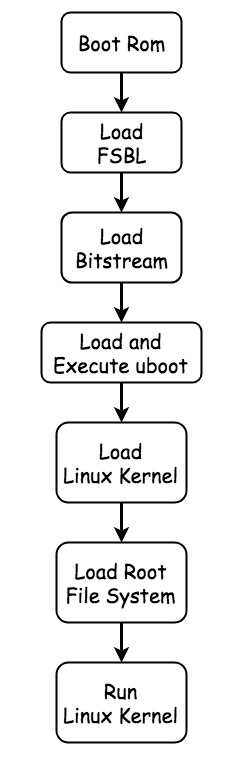
\includegraphics[scale=0.4]{images/linux_boot_stage.jpg}
  \caption[Linux Boot Stage on Target Platform]{Linux Boot Stage on Target Platform}
  \label{fig:Linux Boot Stage on Target Platform}
\end{figure}



\begin{figure}[!htb]
  \centering
  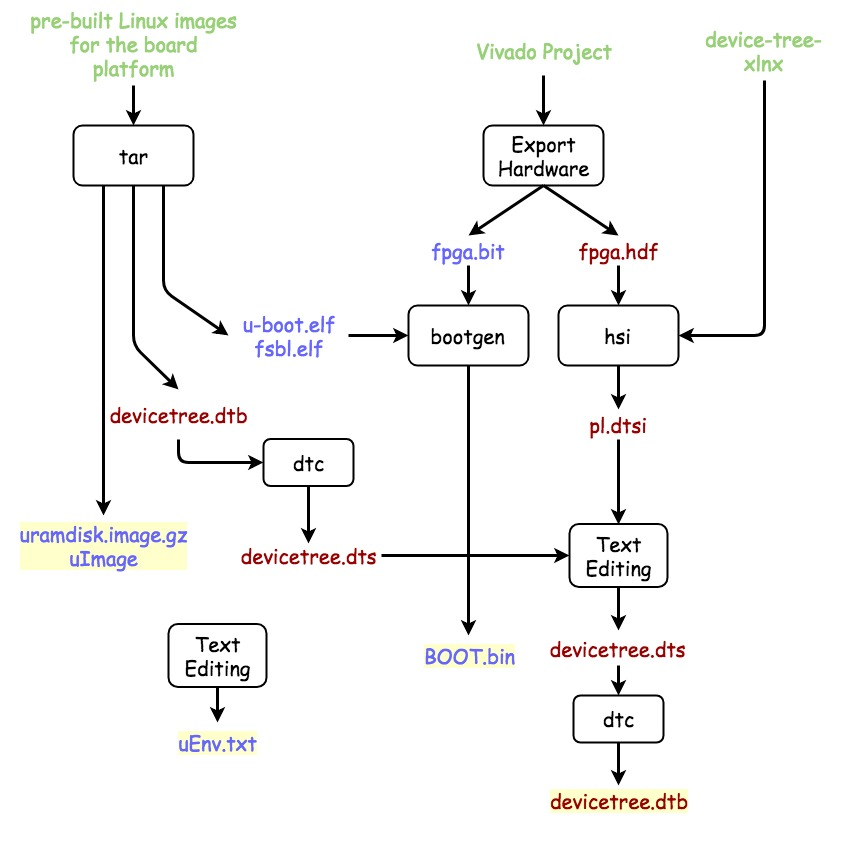
\includegraphics[scale=0.5]{images/embedded_linux.jpg}
  \caption[Embedded Linux on FPGA]{Embedded Linux on FPGA}
  \label{fig:Embedded Linux on FPGA}
\end{figure}

Figure~\ref{fig:Embedded Linux on FPGA} shows an example of how we boot Linux on FPGA\cite{concise}. In this example, we boot Linux on FPGA from SD card, so we need to format SD card into two partitions. The 1st partition is type FAT3, and this partition includes all required boot files, that is BOOT.bin, Linux Kernel(uImage), file system(uramdisk.image.gz), and devicetree file(devicetree.dtb). The 2nd partition is type ext4, and this partition is used as a root file system, so it includes the entire root file system, in our case, we use linaro. 

\subsection{Device Tree}
\label{subsec:Device Tree}

Device Tree is a mechanism to describe all hardware and devices of a system. In early Linux 
kernel, hardware description is hardcoded in kernel files, so porting kernel to a different
platform is painful. To solve this problem, Device Tree is introduced. 
Like x86 based system, we should consider Linux kernel image is a black box, and give the 
hardware information of system to the kernel.
%

In FPGA development flow, the whole system almost keeps the same, the only thing that might change 
is our design in PL(Programmable Logic) side. To boot Linux with different PL design, only 
a little modification of the devicetree file is needed.     


\subsection{Linux Device Driver}
The role of a device driver is a bridge between hardware and software, it communicates with the device and provides functions to applications, like Figure~\ref{fig:Linux Device Driver} shows. A device driver is basically in Linux kernel space, which means if the driver is somehow not working correctly, like getting stuck in an infinite for-loop, the entire system will hang. Hence, a device driver needs to be very robust. 

\begin{figure}[!htb]
  \centering
  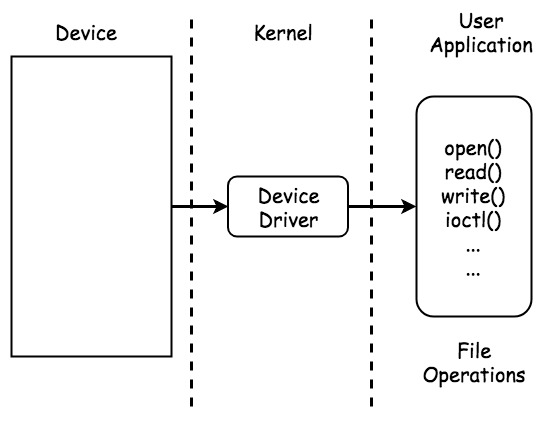
\includegraphics[scale=0.5]{images/linux_device_driver.jpg}
  \caption[Linux Device Driver]{Linux Device Driver}
  \label{fig:Linux Device Driver}
\end{figure}

%-------------------------------------------------------------------------
% Section: UIO driver
%-------------------------------------------------------------------------

\section{UIO}
\label{sec:UIO}
For many types of devices, creating a Linux kernel device driver is overkill. All that is really needed 
is some way to handle an interrupt and provide access to the memory space of the device. To address 
this situation, the userspace I/O system (UIO) was designed. Hardware that is ideally suited for an 
UIO driver fulfills all of the following:
%
\begin{itemize}
\item The device has memory that can be mapped.
\item The device can be controlled completely by writing to this memory.
\item The device usually generates interrupts.
\item The device does not fit into one of the standard kernel subsystems.
\end{itemize}
%
Figure~\ref{fig:UIO Driver} shows how the UIO system works, in software-side of FPGA development, we 
only care about the value in the hardware register and when we can get the correct value, so memory-mapping 
to a userspace application and interrupt handler is really enough in our design flow\cite{howtoUIO}.  
%
\begin{figure}[!htb]
  \centering
  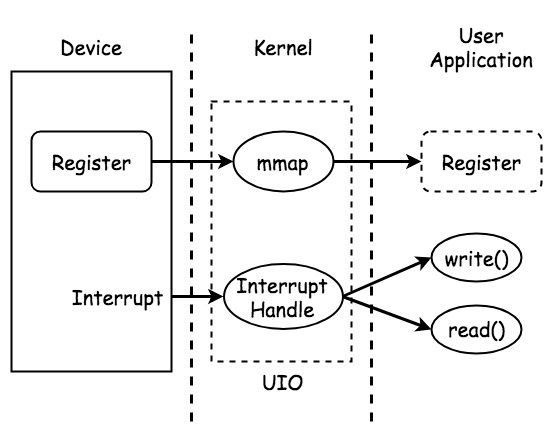
\includegraphics[scale=0.5]{images/uio.jpg}
  \caption[The UIO way.]{The UIO way.}
  \label{fig:UIO Driver}
\end{figure}

%-------------------------------------------------------------------------
% Section: this section may remove because is so hard to explain clearly.
%-------------------------------------------------------------------------
%\section{Register Types in Vivado}
%\label{sec:Register Types in Vivado}

%\begin{itemize}
%\item separate address/control and data phases
%\item support for unaligned data transfers using byte strobes
%\item burst based transactions with only start address issued
%\item issuing of multiple outstanding addresses with out of order responses
%\item easy addition of register stages to provide timing closure.
%\end{itemize}


%\begin{itemize}
%\item AXI4:
%\item AXI4-Lite:
%\item AXI4-Stream:
%\end{itemize}





%-------------------------------------------------------------------------
% Section: DMA
%-------------------------------------------------------------------------
\section{DMA}
\label{sec:DMA}

DMA(Direct Memory Access) is a feature that allows hardware subsystems to access main system memory independent of the CPU. For example, when CPU wants to submit a DMA transaction, it needs to give the DMA controller where the data is(memory address), and size of the data(data length). After submit, the CPU can go back to work for other tasks. Once the transaction is done, the CPU will receive an interrupt from DMA controller and run the callback function.
\begin{figure}[!htb]
  \centering
  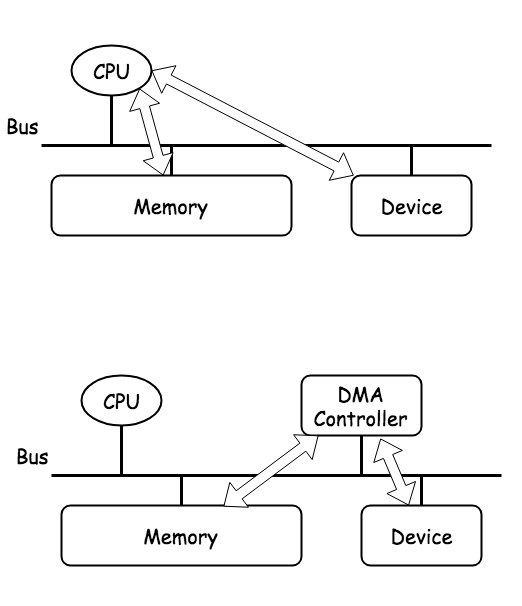
\includegraphics[scale=0.5]{images/DMA.jpg}
  \caption[Direct Memory Access]{Direct Memory Access}
  \label{fig:DMA}
\end{figure}
\newpage
\subsection{DMA Engine }
\label{subsec:DMA Engine}
In real world, we use DMA controller to handle DMA works, by setting value to registers to submit the transactions. But this is in hardware perspective, if we want to use DMA more smartly, we need to abstract this concept to software-level, then there is the ``DMA Engine''. By using the DMA Engine, we can use DMA easily by following the steps below:
\begin{itemize}
\setlength{\itemsep}{0pt}
\item[\textbf{1.}] Request Slave Channel
\item[\textbf{2.}] Set parameters 
\item[\textbf{3.}] Get a descriptor for transaction
\item[\textbf{4.}] Submit the transaction
\item[\textbf{5.}] Issue pending requests and wait for callback notification
\end{itemize}
